%%%% Proceedings format for most of ACM conferences (with the exceptions listed below) and all ICPS volumes.
\documentclass[sigconf]{acmart}
\usepackage{graphicx, wrapfig}
\graphicspath{{imgs/}}
\usepackage[para]{footmisc} %  footnotes na mesma linha
\usepackage{lipsum}
\usepackage{stfloats}
\usepackage{enumerate}
\usepackage[most]{tcolorbox}
\usepackage[english,ngerman,brazilian]{babel}


\newtcolorbox[blend into=figures]{card}[2][]{enhanced,
  float=tbp,title={#2},
  colframe=gray!75!black,olback=yellow!5!white,#1
}


\settopmatter{printacmref=false}
\setcopyright{none}
\renewcommand\footnotetextcopyrightpermission[1]{}
\pagestyle{plain}
\captionsetup{justification   = raggedright,
              singlelinecheck = false}
\newcommand{\source}[2]{\raggedleft{}\vspace*{-7mm}\caption*{ \textmd{\scriptsize{Dados: {#1}.\hfill Ferramenta:{#2}}}}}
\def\BibTeX{{\rm B\kern-.05em{\sc i\kern-.025em b}\kern-.08emT\kern-.1667em\lower.7ex\hbox{E}\kern-.125emX}}

% end of the preamble, start of the body of the document source.
\begin{document}

%
% The "title" command has an optional parameter, allowing the author to define a "short title" to be used in page headers.
\title[Fronteiras da Transferência de Aprendizado: uma revisão sistemática com enfoque meta-analítico]{Fronteiras da Transferência de Aprendizado: \\
uma revisão sistemática com enfoque meta-analítico}
%

\author{Fred Guth}
\email{fredguth@fredguth.com}
\affiliation{%
  \institution{Departamento de Ciência de Computação, Universidade de Brasília}
  \postcode{70.910-900}
  \city{Brasília}
  \state{DF}
  \country{Brazil}
}

\renewcommand{\shortauthors}{Guth, F.}

\begin{abstract}
  Humanos e animais conseguem aprender com poucas amostras e apresentam extraordinária capacidade de generalização que os algoritmos de aprendizagem de máquina ainda estão longe de alcançar~\cite{goodfellow}. Os modelos mais bem sucedidos da atualidade exigem uma enormidade de dados bem rotulados que são caros e difíceis de obter, tornando-se hoje um dos maiores empecilhos para aplicações práticas. Tais fatos apontam para o grande potencial da área de Transferência de Aprendizado, que tem por objetivo aproveitar o conhecimento obtido em uma atividade para aprender mais eficientemente outras, que guardem alguma relação com a primeira. O presente estudo visa apresentar uma revisão sistemática da literatura e identificar, com embasamento quantitativo, as principais contribuições para a área. Além disso, usamos medidas de acoplamento bibliográfico para identificar trabalhos na fronteira do conhecimento e fizemos uma análise textual, em resumos e palavras-chave, comparando estes com os "clássicos" da área de forma a mapear para que direção a pesquisa avança.  
\end{abstract}


\begin{CCSXML}
<ccs2012>
 <concept>
 <concept_id>10010147.10010257.10010258.10010262.10010277</concept_id>
 <concept_desc>Computing methodologies~Transfer learning</concept_desc>
 <concept_significance>500</concept_significance>
 </concept>
</ccs2012>
\end{CCSXML}
\ccsdesc[500]{Computing methodologies~Transfer learning}

\keywords{transferência de aprendizado, revisão sistemática, enfoque meta-analítico}


\maketitle


\section{Introdução} 
  Recentes avanços em Aprendizagem de Máquina tornam possíveis aplicações que são capazes de reconhecer pessoas, lugares e objetos com acurácia super-humana\cite{fei}, diagnosticar câncer de pele tão bem quanto dermatologistas\cite{skin_cancer},  ver através de paredes usando sinais de rádio\cite{wifi}, entre tantas outras. Apesar de tanto sucesso, os modelos mais bem sucedidos da atualidade exigem uma enormidade de dados bem rotulados que são caros e difíceis de obter, pois, em geral, o jeito padrão de se treinar modelos é sempre começar \emph{tabula rasa}, ou seja, com uma inicialização aleatória dos parâmetros~\cite{Ruder2019Neural}. 
  
  Aprender assim, a partir do nada, é contrário à forma como os humanos o fazem. Em nosso dia a dia, transferimos conhecimento a todo momento. Saber tocar piano, facilita aprender tocar órgão. Saber português ajuda a aprender espanhol. Pessoas conseguem inteligentemente aplicar conhecimento prévio para resolver novos problemas com maior eficácia e eficiência\cite{PanYang}. Algoritmos de aprendizagem de máquina ainda estão longe de alcançar essa extraordinária capacidade de generalização\cite{goodfellow}. Estudos recentes~\cite{DBLP:journals/corr/JiaL17}, mostram que os algoritmos atuais não generalizam bem além de dados vistos durante o treinamento. 
  \begin{figure}[h]
    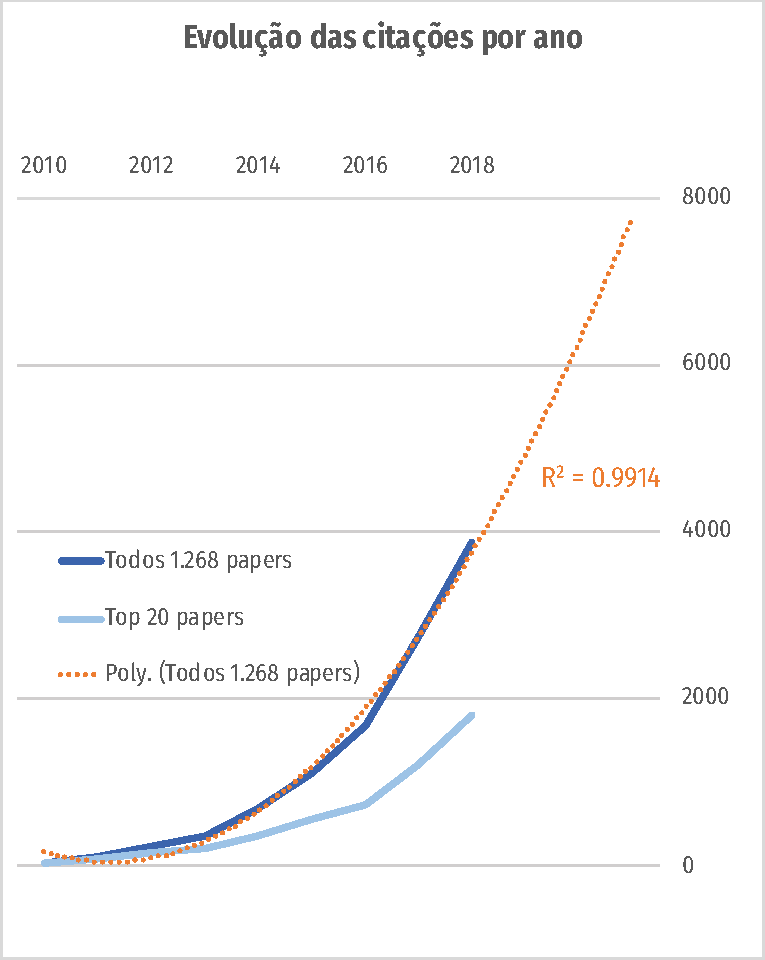
\includegraphics[width=\columnwidth]{citacoes_por_ano}
    \source{Web of Science (março/2019)}{Excel}
    \caption{Evolução do número de citações aos artigos em Tranferência de Aprendizado nos últimos 10 anos. Até 2020, o número de citações aos artigos na área deverá dobrar.}
    \label{fig:citacoes_por_ano}
  \end{figure}

  Tais fatos apontam  o grande potencial ainda inalcançado da área de Transferência de Aprendizado (TL\footnote{Do inglês, \emph{Transfer Learning}.}), que tem por objetivo aproveitar o conhecimento obtido em uma atividade para aprender mais eficientemente outras, que guardem alguma relação com a primeira.
  
  Na prática, entretanto, TL ainda é tratada de uma forma \textit{ad hoc}, sendo os métodos de transferências meras extensões dos algoritmos de aprendizado utilizados \cite{torrey}. Essa dicotomia entre a importância do problema e a inexistência de práticas e teorias consolidadas, tornam TL um campo promissor e interessante para pesquisa. 
  
  \begin{quote} "Transferência de Aprendizado será o próximo motor do sucesso comercial com Aprendizado de Máquinas." \hfill ---Andrew Ng, Tutorial NIPS 2016 \cite{ANg}
  \end{quote}

  Portanto, não é de se estranhar o crescente interesse pelo assunto (vide figura \ref{fig:citacoes_por_ano} e \S\ref{sec:panorama}).  

  \subsection{Objetivo}
   Esta pesquisa quer responder duas perguntas:
    \begin{enumerate}
      \item{Quais são as fronteiras do conhecimento em Transferência de Aprendizado?}
      \item {É possível embasar essa avaliação em dados bibliométricos?}
    \end{enumerate}
    Para responder estas perguntas é preciso, antes, analisar a literatura do tema, revelar as principais contribuições na área e como se relacionam.
  
  \subsection{Contribuições}

    \begin{enumerate}[C1.]
      \item Apresentamos uma revisão sistemática atualizada da literatura em Transferência de Aprendizagem, usando a abordagem TEMAC (\S \ref{TEMAC}). Esse método nos permite focar nas contribuições de alto impacto. 
      \item Estendemos o TEMAC com uma análise textual de resumos (\S \ref{analiseTextual}), utilizando o \emph{ScatterText}~\cite{kessler2017scattertext}, o que até onde sabemos, é uma aplicação original desta ferramenta de visualização.
      \item Apontamos com embasamento quantitativo as direções das frentes de pesquisa da área e apontamos lacunas e problemas em aberto.
    \end{enumerate}
  
  \subsection{Visão Geral e Organização do Artigo}
  \lipsum[3]
  \subsection{Trabalhos Relacionados}
  \lipsum[2]
\section{Método: Revisão com Enfoque Meta-Analítico Consolidado}\label{TEMAC}
Na presente pequisa utilizamos o método de revisão sistemática da Teoria do Enfoque Meta-Analítico (TEMAC) ~\cite{Mariano}, que visa oferecer um embasamento quantitativo para a escolha da literatura. Apesar do nome, TEMAC não deve ser confundida com Meta-Análise, pois o foco desta é gerar conhecimento por meio de dados empíricos secundários, enquanto o daquela é oferecer uma sistematização da escolha bibliográfica.

A abordagem TEMAC é dividida em 3 etapas: 
\begin{enumerate}[a)]
  \item preparação da pesquisa;
  \item apresentação e inter-relação dos dados;
  \item detalhamento, modelo integrador e validação por evidências.
\end{enumerate}

\subsection{Preparação da Pesquisa}
Foi realizada uma busca na base de dados \emph{Clarivate Analyticis Web of Science (WoS)}, conforme especificado na figura \ref{card:wos}, no dia 31 de março de 2019, que resultou em 1.289 artigos encontrados. Nota-se que o tema é de crescente interesse (figura \ref{fig:citacoes_por_ano}) e projeta-se que em 2 anos o número de citações irá praticamente dobrar (crescimento cubico com R-quadrado 0,9993). 
\begin{figure}[htp]

\begin{tcolorbox}[colback=yellow!5!white,colframe=gray!75!black,title={Results: 1,289 (from Web of Science Core Collection)}]
  \footnotesize{
    \begin{verbatim}
    You searched for: 
    TOPIC: ("transfer learning")
    Refined by: 
    WEB OF SCIENCE CATEGORIES: 
      ( COMPUTER SCIENCE ARTIFICIAL INTELLIGENCE )
    AND LANGUAGES: ( ENGLISH ) 
    AND RESEARCH AREAS: ( COMPUTER SCIENCE )
    Timespan: 2009-2019. 
    Indexes: SCI-EXPANDED, CPCI-S, ESCI.
    \end{verbatim}
  }

\end{tcolorbox}
\caption{"Busca10anos": Parâmetros de busca na base \emph{Web of Science}.}
\label{card:wos}
\end{figure}

Também fizemos uma busca mais restrita aos trabalhos mais recentes (figura \ref{card:sota}) para a análise da \emph{Fronteira de Pesquisa} (\S \ref{fronteira}).
\begin{figure}[htp]
  \begin{tcolorbox}[colback=yellow!5!white,colframe=gray!75!black,title={Results: 384 (from Web of Science Core Collection)}]
    \footnotesize{
  \begin{verbatim}
  You searched for: 
  TOPIC: ("transfer learning")
  Refined by: 
  WEB OF SCIENCE CATEGORIES: 
    ( COMPUTER SCIENCE ARTIFICIAL INTELLIGENCE )
  AND LANGUAGES: ( ENGLISH ) 
  AND RESEARCH AREAS: ( COMPUTER SCIENCE )
  AND PUBLICATION YEARS: ( 2019 OR 2018 OR 2017 )
  AND DOCUMENT TYPES: ( PROCEEDINGS PAPER )
  Timespan: 2009-2019. 
  Indexes: SCI-EXPANDED, CPCI-S, ESCI.
  \end{verbatim}
    }
  
  \end{tcolorbox}
  \caption{"Busca2anos"Parâmetros de busca para análise de Fronteira.}
  \label{card:sota}
\end{figure}

\subsection{Apresentação e Inter-relação dos Dados}

% O software livre \emph{VosViewer 1.6.10}~\cite{VOSviewer} foi utilizado para as análises bibliográficas. Ele permite analisar co-citação e acoplamento bibliográfico de documentos e autores. Para análise textual de resumos utilizamos a ferramenta \emph{ScatterText}~\cite{kessler2017scattertext}.

\begin{enumerate}[a)]
  \item{\textbf{Análise de Co-citações}: Co-citação é definida como a frequência em que dois documentos são citados em uma mesma lista de referências. Assume-se que são "peças"~que compõem uma mesma "estrutura de conhecimento".  A análise de co-citações, portanto, é útil para mapear a herança intelectual de um determinado campo de estudos sob a ótica das publicações de alto-impacto, mas tende a negligenciar a dinâmica na fronteira de pesquisa\cite{Vogel2012}, justamente porque os trabalhos na fronteira não tiveram tempo para serem citados e pontuar nas métricas de impacto.\\Para a análise de co-citações, utilizamos o software livre \emph{VosViewer 1.6.10}~\cite{VOSviewer}, que \emph{clusterizou} citações das listas de referências dos artigos da "Busca10anos" (o que abrange artigos que não fazem parte do resultado da busca). Foram identificados 3 núcleos de conhecimento (figura \ref{fig:classicos}).
  }

  \item{\textbf{Análise de Acoplamento Bibliográfico}: Acoplamento bibliográfico ocorre quando dois documentos tem pelo menos um documento em comum, ou seja, documentos acoplam se suas bibliografias se sobrepõem. Como existe uma ordem cronológica entre o documento que cita e o que é citado, o acoplamento bibliográfico permite traçar gerações de pesquisas e com isso identificar as que estão na fronteira do conhecimento.  É importante ressaltar que, neste contexto, estar na fronteira não é necessariamente ser promissor. Essa é uma limitação da abordagem quantitativa, por isso é preciso complementá-la com uma análise qualitativa para propor, ainda que com certo grau de subjetividade, os trabalhos promissores a se tornar os "clássicos de amanhã". \\Pelo TEMAC, a análise de acoplamento bibliográfico deve ser feita para o período um período não superior aos últimos 3 anos. Em nossa análise, usamos uma busca mais restrita (figura \ref{card:sota}) com período entre 2018 e março de 2019.
  }
  \item{\textbf{Análise Textual (\emph{bag-of-words}  com tf-idf)}: nesta análise, tratamos os artigos como \emph{bag-of-words} e usamos o conceito de \textbf{tf-idf} para definir as palavras (termos) que melhor identificam determinados artigos (documentos). Por exemplo, quais palavras melhor explicam trabalhos de fronteira vis à vis o todos os documentos resultantes da busca na base \emph{Web of Science} (vide figura \ref{fig:scatterText}. A métrica \textbf{tf-idf} pode ser definida como:
  \begin{equation}
    \mathrm{tfidf}(t,d,D) = \mathrm{tf}(t,d) \cdot \mathrm{idf}(t, D)
  \end{equation}
  onde $\mathrm{tf}(t,d)$ é a frequência em que um termo $t$ aparece em um documento $d$ e $\mathrm{idf}(t, D)$ é o inverso da frequência do termo $t$ no conjunto de documentos $D$ (o \emph{corpus}). 
  \begin{equation}
    \mathrm{tf}(t,d) = 0.5 + 0.5 \cdot  \frac{f_{t, d}}{\max\{f_{t', d}:t' \in d\}}
  \end{equation}
  \begin{equation}
    \mathrm{idf}(t, D) =  \log \frac{N}{|\{d \in D: t \in d\}|}
  \end{equation}
  onde:
  \begin{description}
    \item $N$: número de documentos do corpus $N = {|D|}$
   \item$ |\{d \in D: t \in d\}| $ : número de documentos onde o termo  $ t $ aparece (i.e., $ \mathrm{tf}(t,d) \neq 0$). Para evitar uma divisão por zero caso o termo não esteja no corpus, é como fazer um ajuste no denominador para: $1 + |\{d \in D: t \in d\}|$.
  \end{description}
  
  A métrica \textbf{tf-idf} é a base da ferramenta visual \emph{ScatterText}~\cite{kessler2017scattertext} que foi utilizada para gerar as figuras \ref{fig:scatterText_documentbased} e \ref{fig:scatterText}.

  }\label{analiseTextual}
\end{enumerate}



\section{Revisão da Literatura}
  \subsection{Um breve histórico}
  Pesquisa em transferência de aprendizado tem atraído mais e mais atenção desde 1995, quando foi tema de  um workshop na NIPS-95 que discutiu a necessidade de métodos de aprendizado de máquina que retém e reusam conhecimento previamente obtido~\cite{PanYang}. 
  
  Desde então, ainda que com diferentes nomes (\emph{learning to learn, life-long learning, knowledge transfer} entre outros), a área vem recebendo cada vez mais atenção (figura \ref{fig:artigos_por_ano}). Em 2005 um anúncio de um projeto da DARPA foi a primeira menção que definia o termo \emph{transfer learning} como o objetivo de extrair conhecimento de um ou mais \emph{tarefas fonte} e aplicá-lo a \emph{tarefas alvo}~\cite{PanYang}. Se removermos a restrição de data de início da "Busca10Anos"(figure \ref{card:wos}), confirmamos que os primeiros artigos com o termo "transfer learning" são de 2005.

  \begin{figure}[h]
    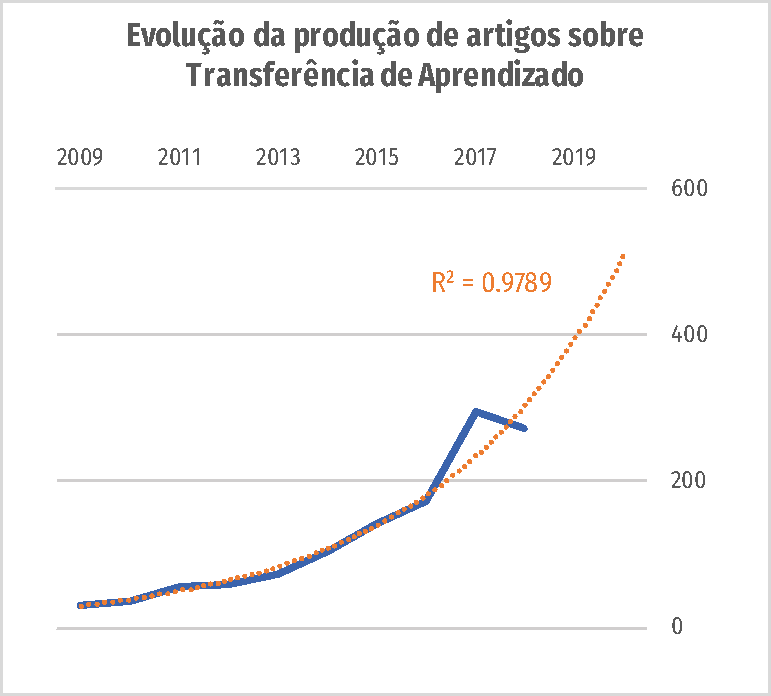
\includegraphics[width=\columnwidth]{artigos_por_ano}
    \source{Web of Science (março/2019)}{Excel}
    \caption{Evolução do número de artigos em Tranferência de Aprendizado nos últimos 10 anos. Até 2021, o número de artigos na área deverá dobrar.}
    \label{fig:artigos_por_ano}
  \end{figure}

  Em 2012, a rede neural profunda\footnote{deep neural network} submetida pelo time de Alex Krizhevsky et. al. para o desafio Imagenet (ILSVRC) performou 41\% melhor que o segundo melhor colocado, dando início ao crescimento explosivo de \emph{deep learning"} na pesquisa de Aprendizado de Máquinas. Tal sucesso ressaltou a importância dos dados para o avança de inteligência artificial, mas também permitiu uma igual quebra de paradigma em transferência de aprendizado: percebeu-se que modelos treinados na ImageNet podiam facilmente ser usados para inicializar outros modelos e reduzir em muito a necessidade de amostras~\cite{Ruder2019Neural}.   Essa abordagem de "sintonia fina"\footnote{\emph{fine-tuning}} permitiu resultados bons em diversas tarefas com ordens de magnitude a menos de dados. 

  Atualmente, \emph{transferência de aprendizado} é um tópico comum em prestigiadas conferências como CVPR, ICCV, ICPR e NeurIPS (vide figura \ref{fig:toptop}, \emph{Top 10 encontros}).
  \subsection{Notações e definições}
  \subsection{O panorama da produção científica na área}\label{sec:panorama}
  \begin{figure*}[t]
    \centering
    \fbox{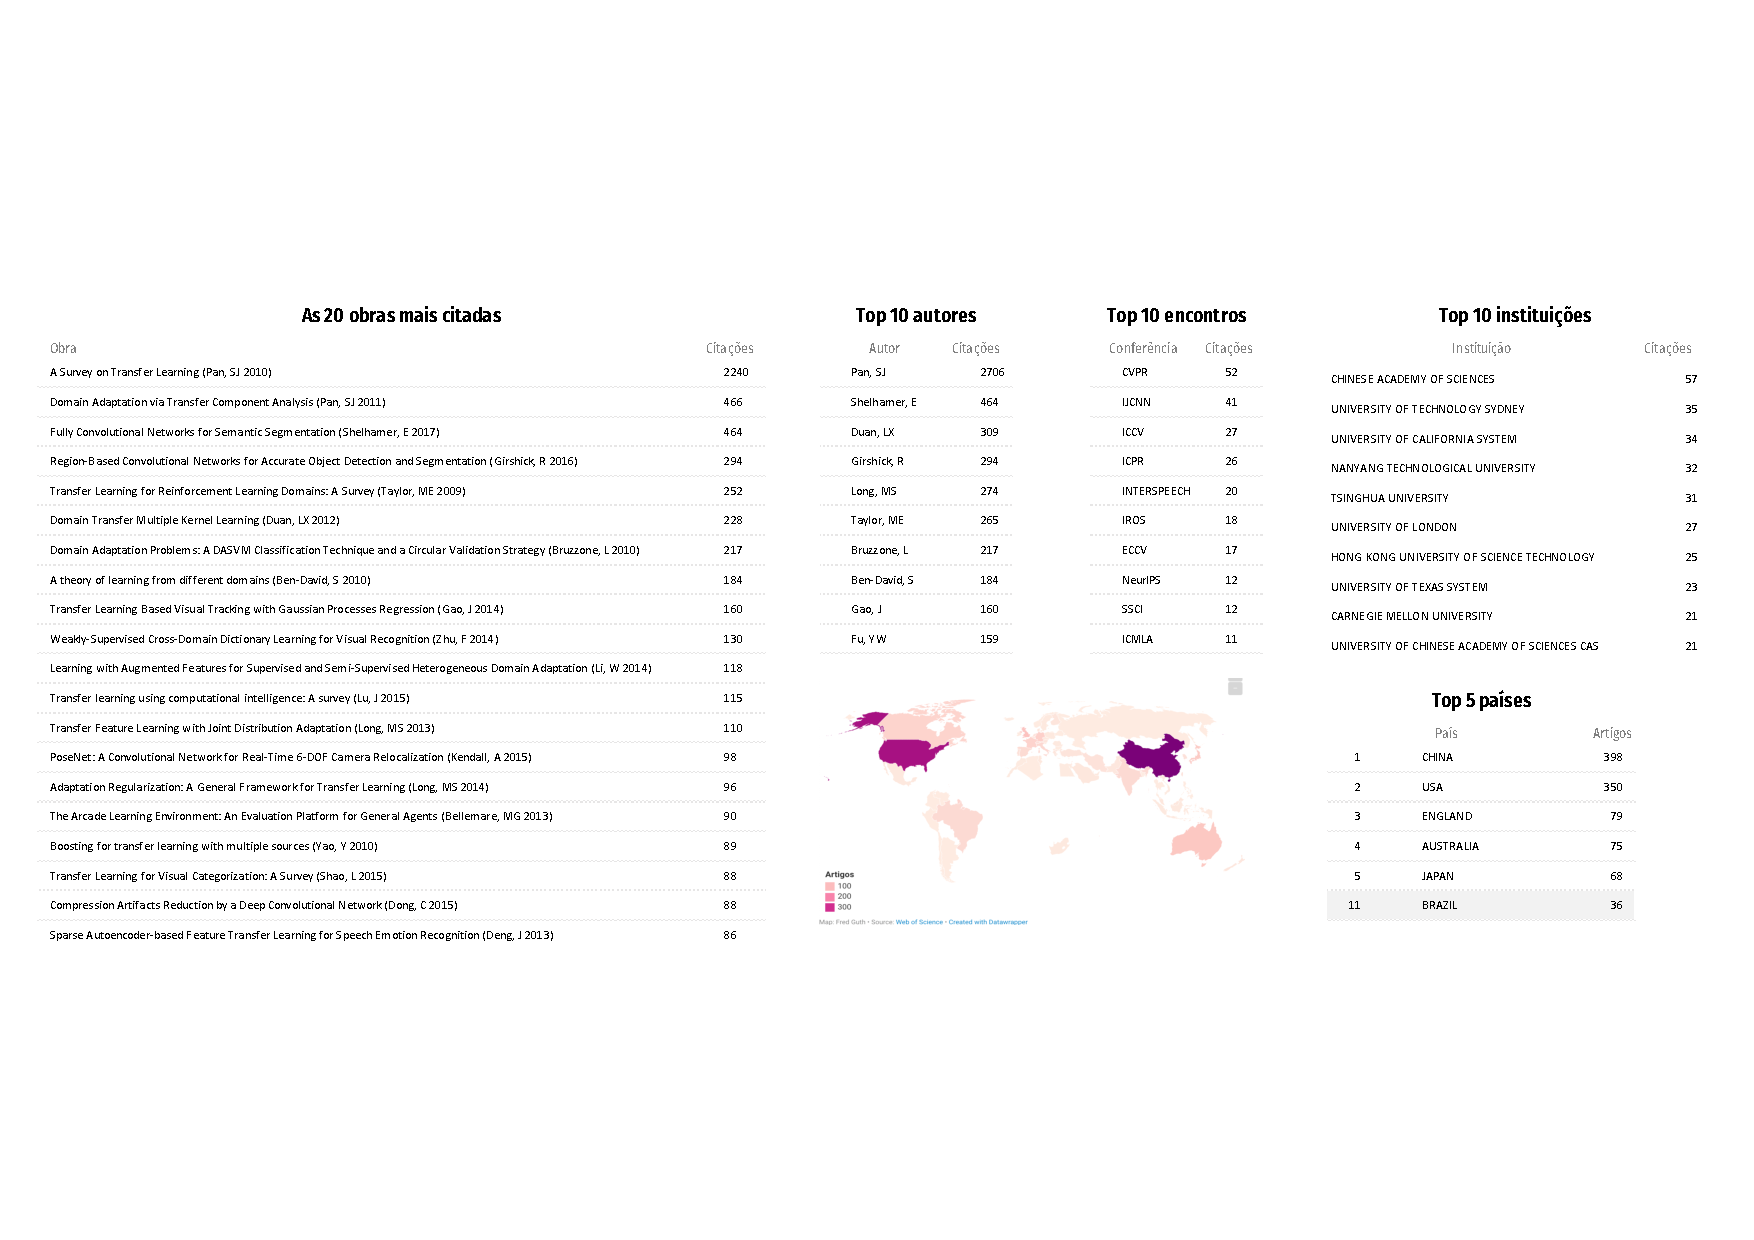
\includegraphics[width=\textwidth]{listas.pdf}}
    \source{Web of Science (março/2019)}{Excel}
    \caption{Panorama da produção científica sobre Transferência de Aprendizado.} \label{fig:toptop}
  \end{figure*}
  Na figura \ref{fig:toptop}, é possível notar que o autor com mais citações é Pan, S., com 2706 citações. Tal impacto deve-se, sobretudo ao artigo \emph{A Survey on Transfer Learning}, que é o artigo mais citado da área com 2240 citações. O mérito deste trabalho é apresentar notações e uma taxonomia para TL. Saiu na revista \emph{IEEE Transactions on Knowledge an Data Engineering}, de 2,775 de fator de impacto, e ocupa a 33\textordfeminine ~posição no ranking de publicações InCite JCR para a categoria \emph{Computer Science, Artificial Intelligence}, ou seja, uma publicação cujo foco não é o tipo de pesquisa que menciona \emph{transferência de aprendizado}. 

  A China é o país com o maior número de artigos publicados, seguido pelos Estados Unidos. O Brazil está na 11\textordfeminine colocação, junto com a Índia, mas a frente de países como Espanha, Coreia do Sul e Israel.

  A maior parte dos artigos são publicados em \emph{proceeding} de conferências, 63\%. A conferência com mais artigos sobre TL é a CVPR\footnote{Conference on Computer Vision and Pattern Recognition}, mas apesar de ser somente a 4\textordfeminine em artigos a ECCV\footnote{European Conference on Computer Vision} é a conferência com o maior número agregado de citações. É digno de nota que as conferências de visão computacional tem sido o espaço onde artigos de TL mais são divulgados. Ao mesmo tempo, estranha a falta de alguma conferência com maior foco em NLP. Também não há entre os 20 artigos mais citados, nenhum que seja especializado em linguagem.
  \subsection{Os Clássicos}\label{classicos}
  \begin{figure}[htp]
    \fbox{\includegraphics[width=\columnwidth]{completo_21.pdf}}
    \source{Web of Science (março/2019)}{VosViewer\protect{~\cite{VOSviewer}}}
    \caption{Núcleos de conhecimento obtidos pela análise de co-citações. Os diferentes grupos representam autores que normalmente são co-citados nos 1268 artigos resultantes da busca realizada.}
    \label{fig:classicos}
  \end{figure}

A análise de co-citação usando o \emph{VosViewer} apontou para existência de 3 núcleos\footnote{\emph{clusters}} de conhecimento. Esses núcleos têm um forte componente temporal, podendo ser vistos como ondas, a primeira concentrando obras anteriores a 2011 (a moda é 2006),  está em amarelo na figura \ref{fig:classicos}, a segunda entre 2011 e 2014 (a moda é 2012) está em vermelho, e a terceira e última onda, em verde na figura, são obras de 2012 até hoje (moda 2014).
\subsubsection{Primeira onda}
Uma das características mais fortes desta onda é sua componente teórica. Nesse núcleo estão obras que apresentam algumas classes de transferência de aprendizado: Thurn, S. (1996) \cite{thrun1996learning} e Caruana, R. (1997) \cite{Caruana1997} introduzem \emph{Multi-Task Learning} e a ideia de que tarefas adicionais (ou auxiliares) introduzem um viés indutivo que facilita a convergência do aprendizado; Chapelle, O. (2006) \cite{Chapelle:2010:SL:1841234} com seu livro sobre \emph{Semi-Supervised Learning}; Raina, R. (2007) e \emph{Self-taught learning}; Vapnik, V. (1998) \cite{Vapnik1998} e os fundamentos da teoria de aprendizagem estatística.
Uma outra componente da primeira onda são artigos de Adaptação de Domínio, com certo foco em abordagens que buscam aprender características latentes, de menor dimensionalidade, com o pressuposto que em um espaço latente os domínios são mais similares: Ando, R. K.(2005) \cite{ando2005framework} e Daume, H.. (2006) \cite{DaumeIII2006}, por exemplo. 
Por fim, algumas das obras mais citadas desta onda são \emph{surveys}: Pan, S. (2010) \cite{PanYang}, Taylor, M. E. (2009) \cite{Taylor:2009:TLR:1577069.1755839}; que não por coincidência aparecem já mais para o final da primeira onda, organizando a pesquisa até aquele ponto. 


ando rk (2005) - project data into low-dimension space to make domains more similar - SVD----- cluster:1
daume h (2006) - latent feature learningDA for statistica lassifiers ----- cluster:1



yao y (2010) - boosting -> domain adaptation ----- cluster:1


  cluster 1 - amarelo
  mediana e moda 2006
  dai w. (2007) - boosting -> domain adaptation ----- cluster:1

  pan sj (2010) - surey----- cluster:1
  taylor me (2009) - survey TL in RL----- cluster:1
chang cc (2011) - LIBSVM: A library for support vector machines----- cluster:1

  cluster 2 - vermelho
  moda 2012
  mediana 2011,5
  pan sj (2011) - DA with TCA -> feature represenation ----- cluster:2
gong bq (2012) - unsupervised domain adaptation----- cluster:2
duan lx (2012) - SVM classifiers DA - cross domain learning----- cluster:2
bruzzone l (2010) - DA SVM -> accuracy assessment for validating learning when no labels of target domain----- cluster:2
si s (2010) - minimize divergence -> domain adaptation----- cluster:2
yang j. (2007) - DA for video using adaptive SVMs----- cluster:2
long ms (2014) - adaptaion regularization - adaptive classifier----- cluster:2
fernando b (2013) - unsupervised domain adaptation----- cluster:2
long ms (2013) - adaptive classifier----- cluster:2
ben-david s (2010) - distribution similarity----- cluster:2

cluster 3 - verde
  moda ano de 2014
  mediana 2013,5
  he km (2016) - He, 2017 = object detection----- cluster:3
  krizhevsky a (2012) - alexnet----- cluster:3
  simonyan k. (2014) - Human tracking using CNN----- cluster:3
  russakovsky o (2015) - Imagenet----- cluster:3
  lecun y (2015) - deep learning----- cluster:3
  oquab m (2014) - Transfer learning -> sequential learning -> fine tunning----- cluster:3
  donahue j. (2014) - parametros aprendidos servem como representacoes universais que permitem aprender com poucos exemplos na tarefa alvo.----- cluster:3
  jia y. (2014) - Caffe framework----- cluster:3
  girshick r (2014) - RCNN - object detection----- cluster:3
  deng j (2009) - Imagenet----- cluster:3
  bengio y (2009) - curriculum learning -> simple to complex representations----- cluster:3
  jia y. (2014) - Adam----- cluster:3
  everingham m (2010) - Pascal VOC----- cluster:3
  long j (2015) - FCN for semantic segmentation----- cluster:3
  bengio y (2013) - review representation learning----- cluster:3
  dalal n (2005) - human detection----- cluster:3
  glorot x. (2011) - proposed first approach that applied a deep neural netwok to learn a common representaiton for domain adaptation  SDA----- cluster:3
  hinton ge (2006) - deep learning----- cluster:3
  kingma d. (2014) - alexnet----- cluster:3
  felzenszwalb pf (2010) - Object Detection----- cluster:3


  Sequential Transfer Learning became ubiquituous -> not using is considered foolhardy mahajan, 2018 ->descuidado
  squential learning is commonly as pretraining ImageNEt -> Deng, 2009
  Donahue, 2014 -> parametros aprendidos servem como representacoes universais que permitem aprender com poucos exemplos na tarefa alvo.

  pre-treained -> sota results in several tasks -> He, 2017 = object detection -> Zhao, 2017 semantic segmentation, Papandreaou , 2017 human pose esimation.
  Deng et al, 2013 -> MTL for speech Recognition
  Caruana, MTL introduces an inductive bias provided by the auxiliary tasks ->chapter on multitask learning - hard parameter sharing
  Taylor -> survey of tL in RL
  Duong 2015, MTL soft parameter sharing
  wang and zheng 2015, Sequential transfer leanring => model transfer
networks.


  Domain adaptation
  Jiang, 2008 - survey
  zhou 2014, 2015 -> different feature spaces 
  weightning approaches Huang, 2007, Sugiama 2008
      


  
  \begin{figure}
    \fbox{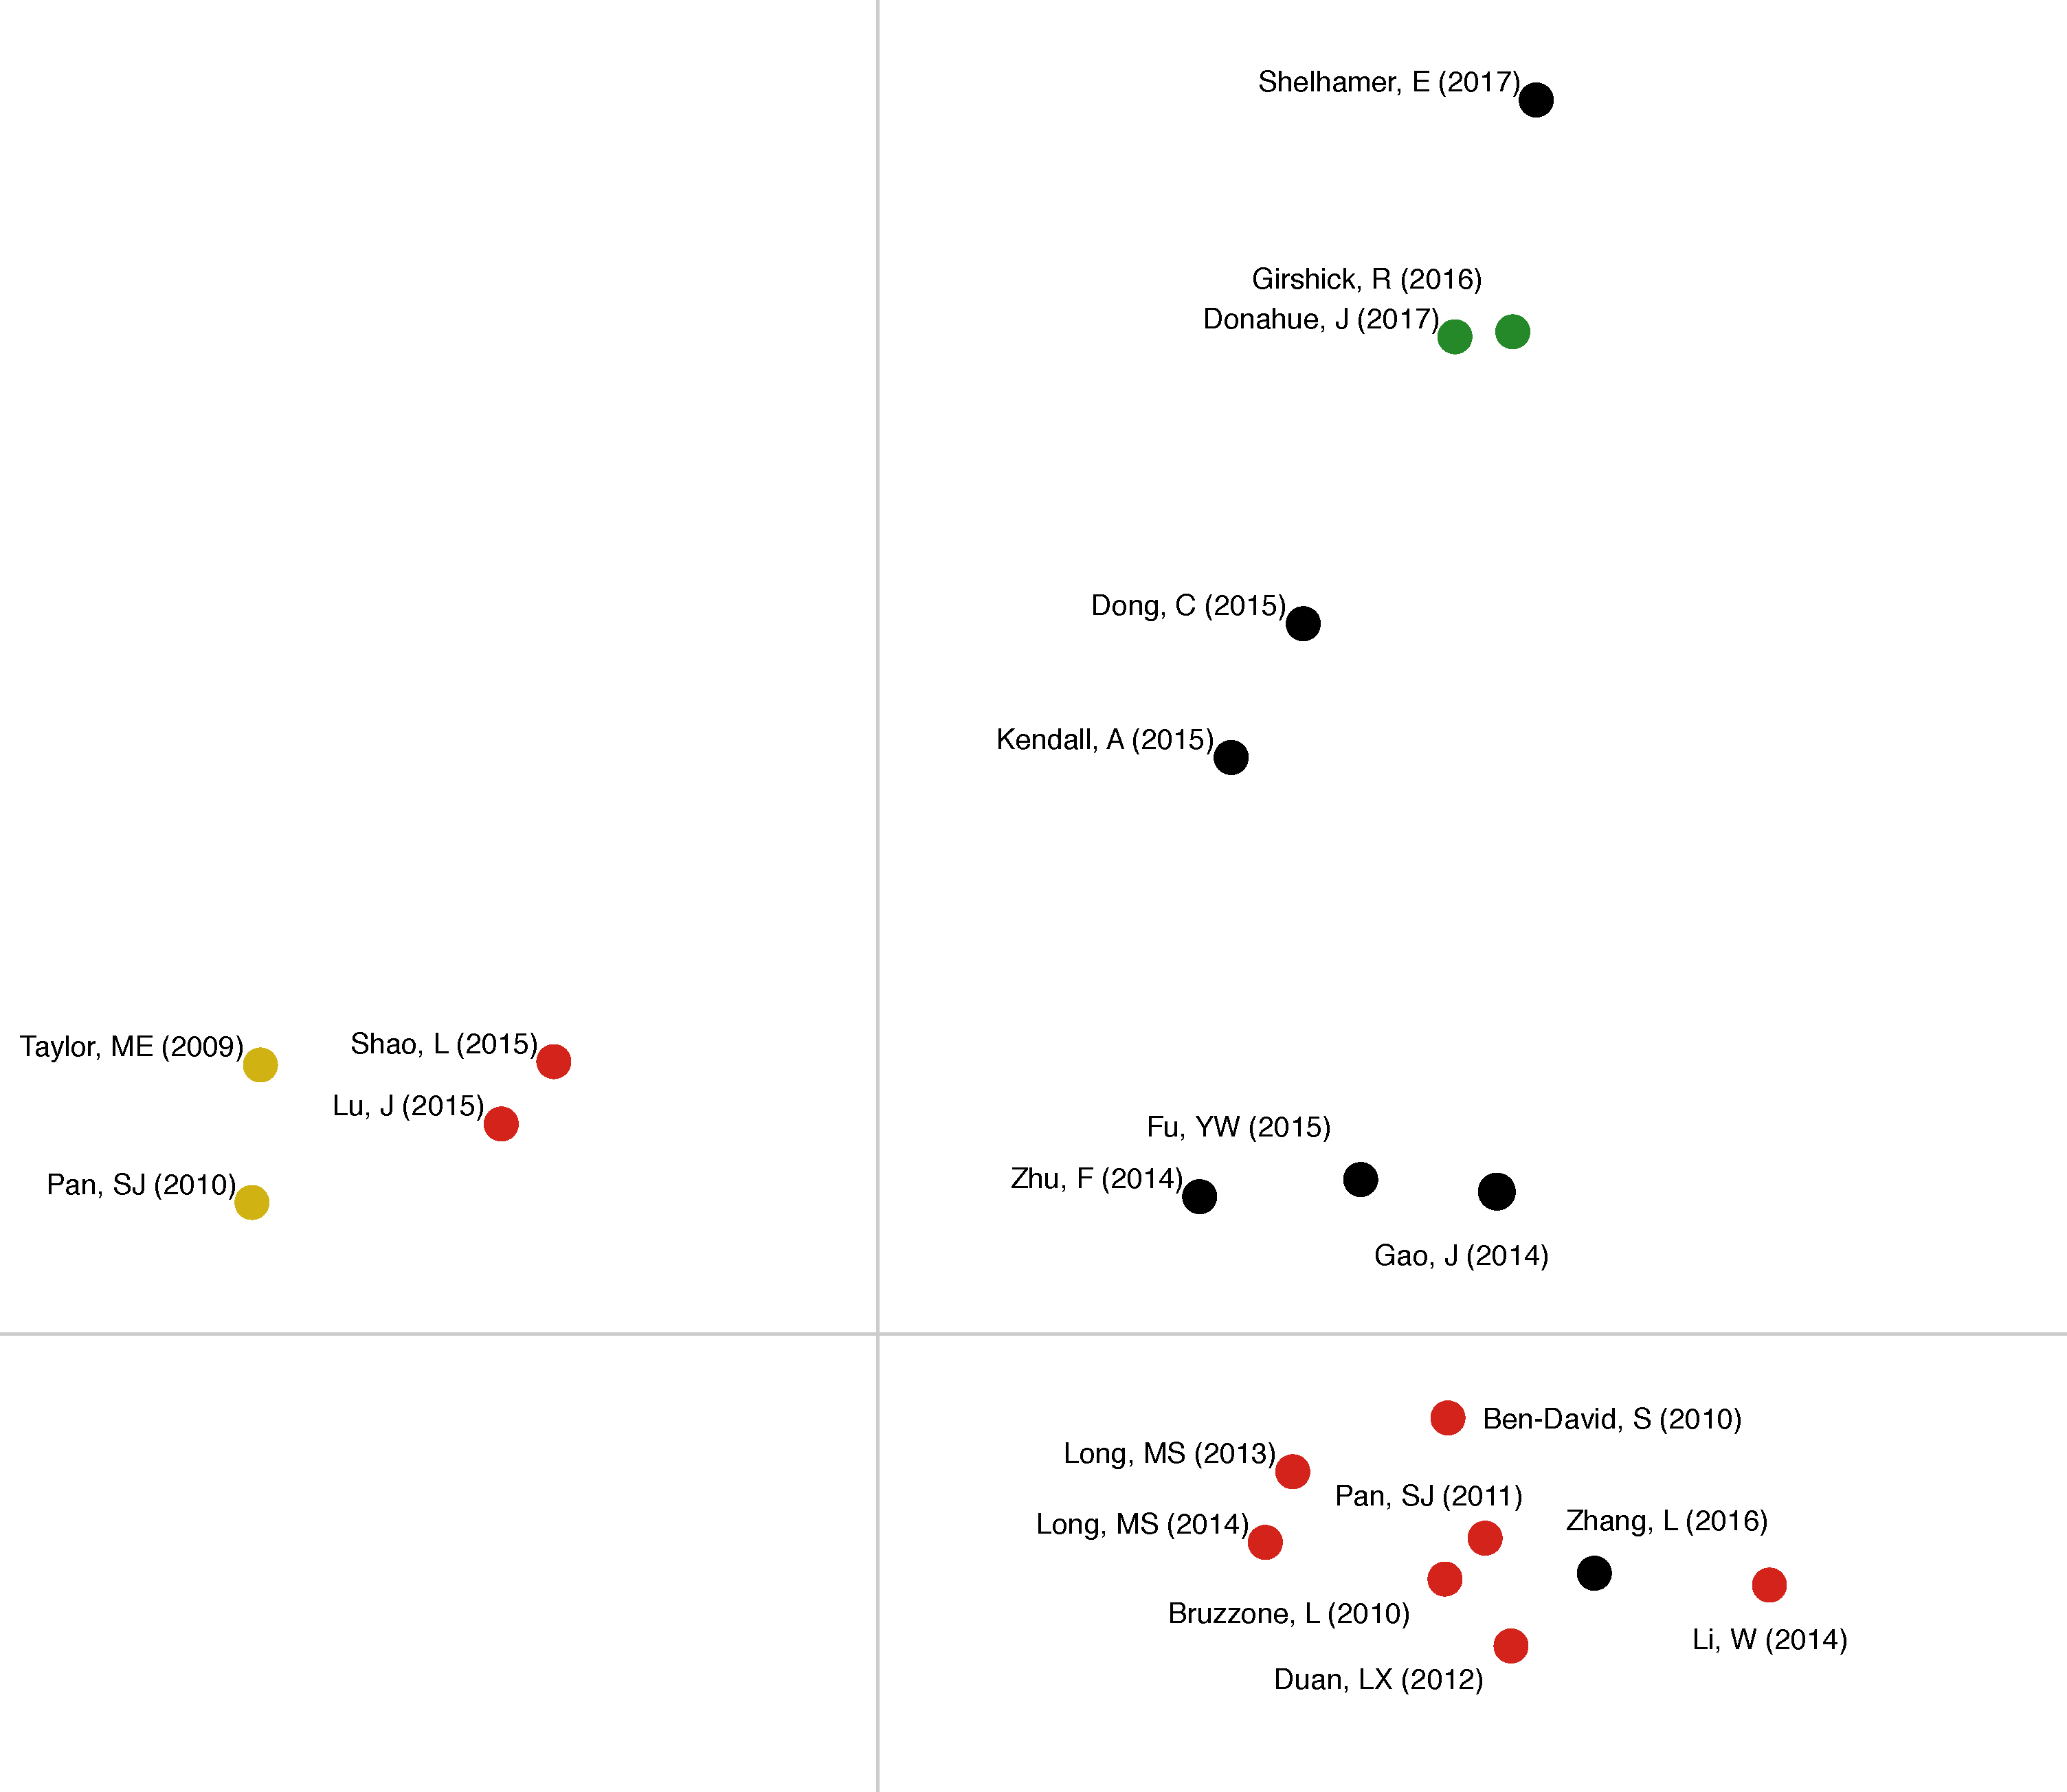
\includegraphics[width=\columnwidth]{top20_abstracts.pdf}}
    \caption{} \label{fig:scatterText_documentbased}
  \end{figure}
  \begin{figure}
    \fbox{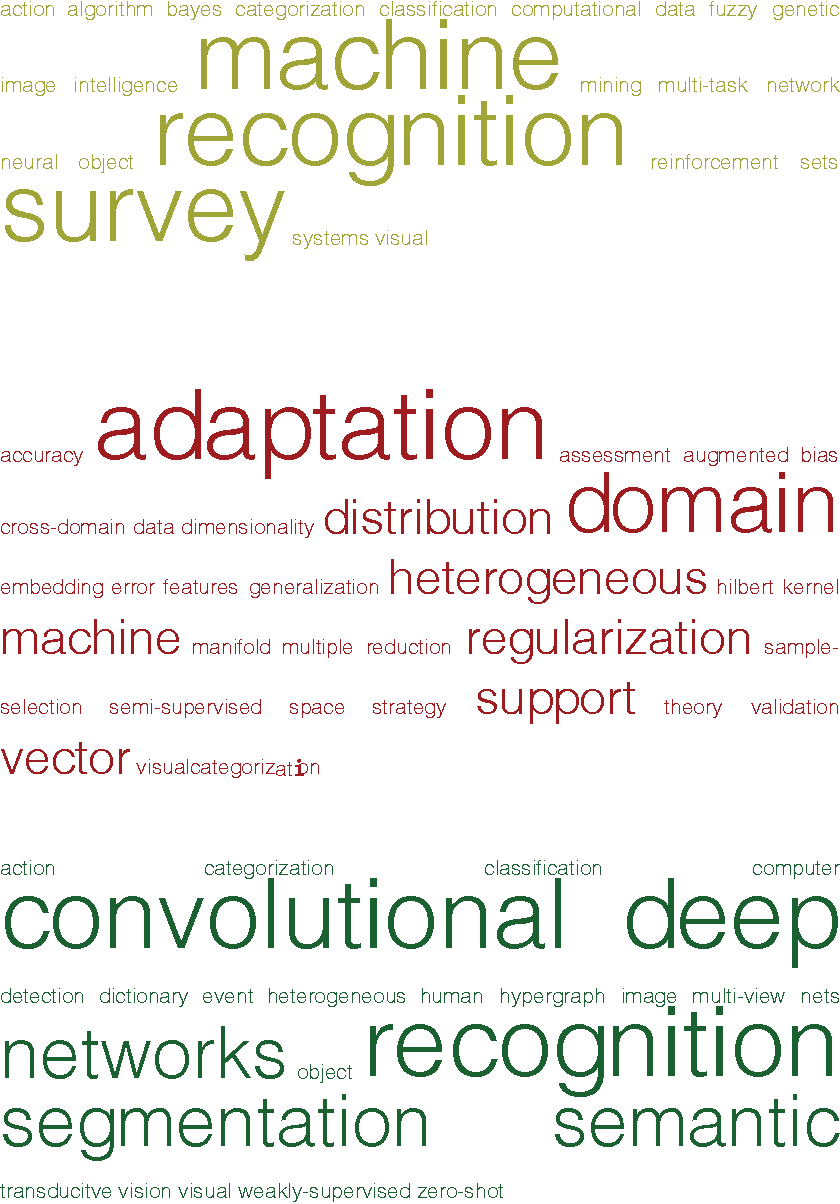
\includegraphics[width=\columnwidth]{keyword_clouds}}
    \caption{} \label{fig:clouds}
  \end{figure}
  \subsection{A Fronteira}\label{fronteira}
  \lipsum[2]
  \begin{figure}
    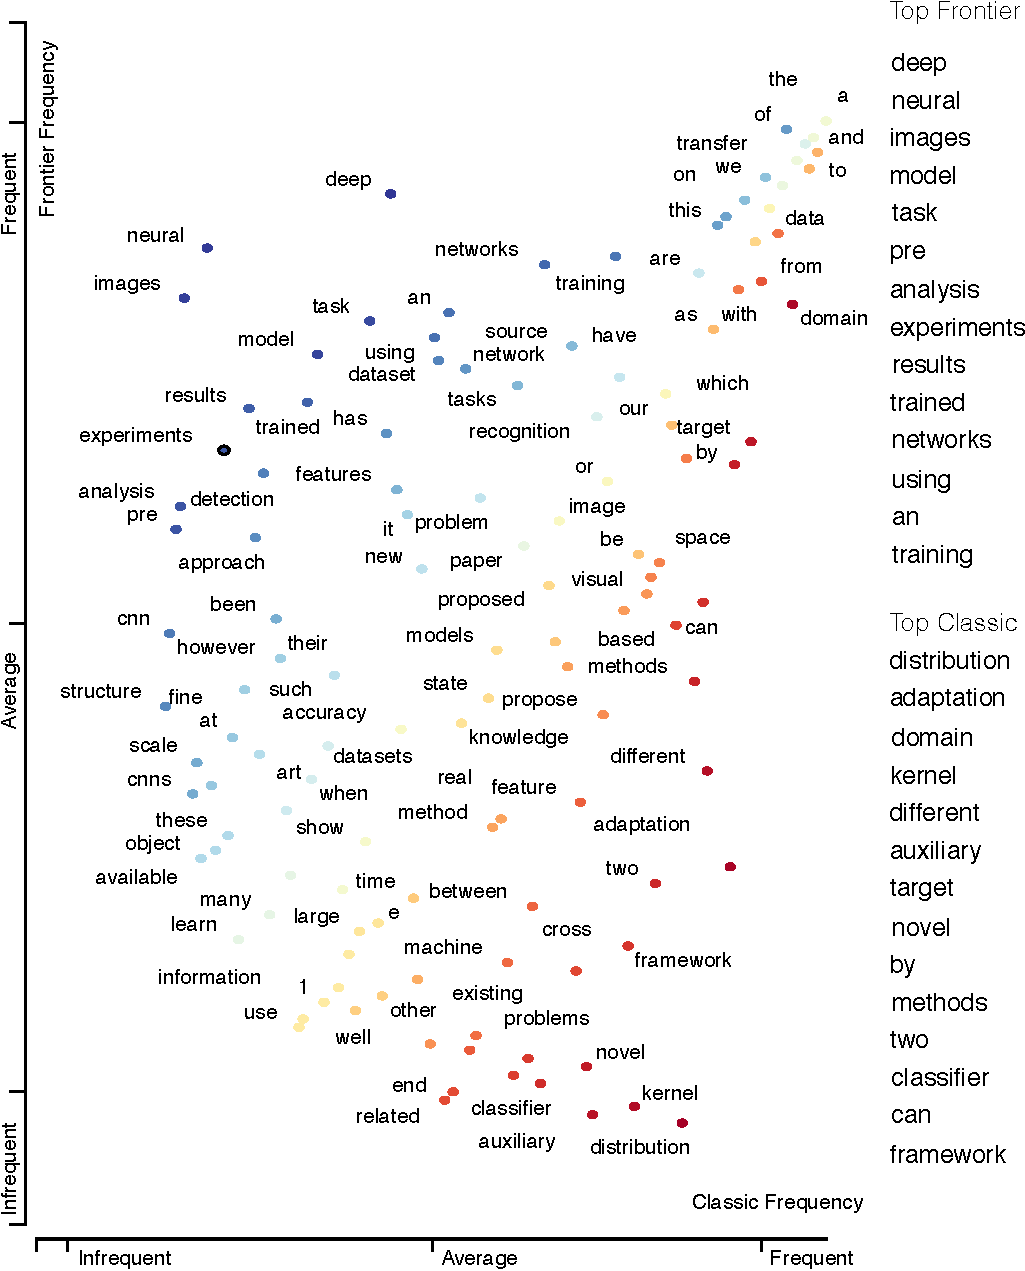
\includegraphics[width=\columnwidth]{frontier3.pdf}
    \caption{} \label{fig:scatterText}
  \end{figure}
  \begin{figure}
    \fbox{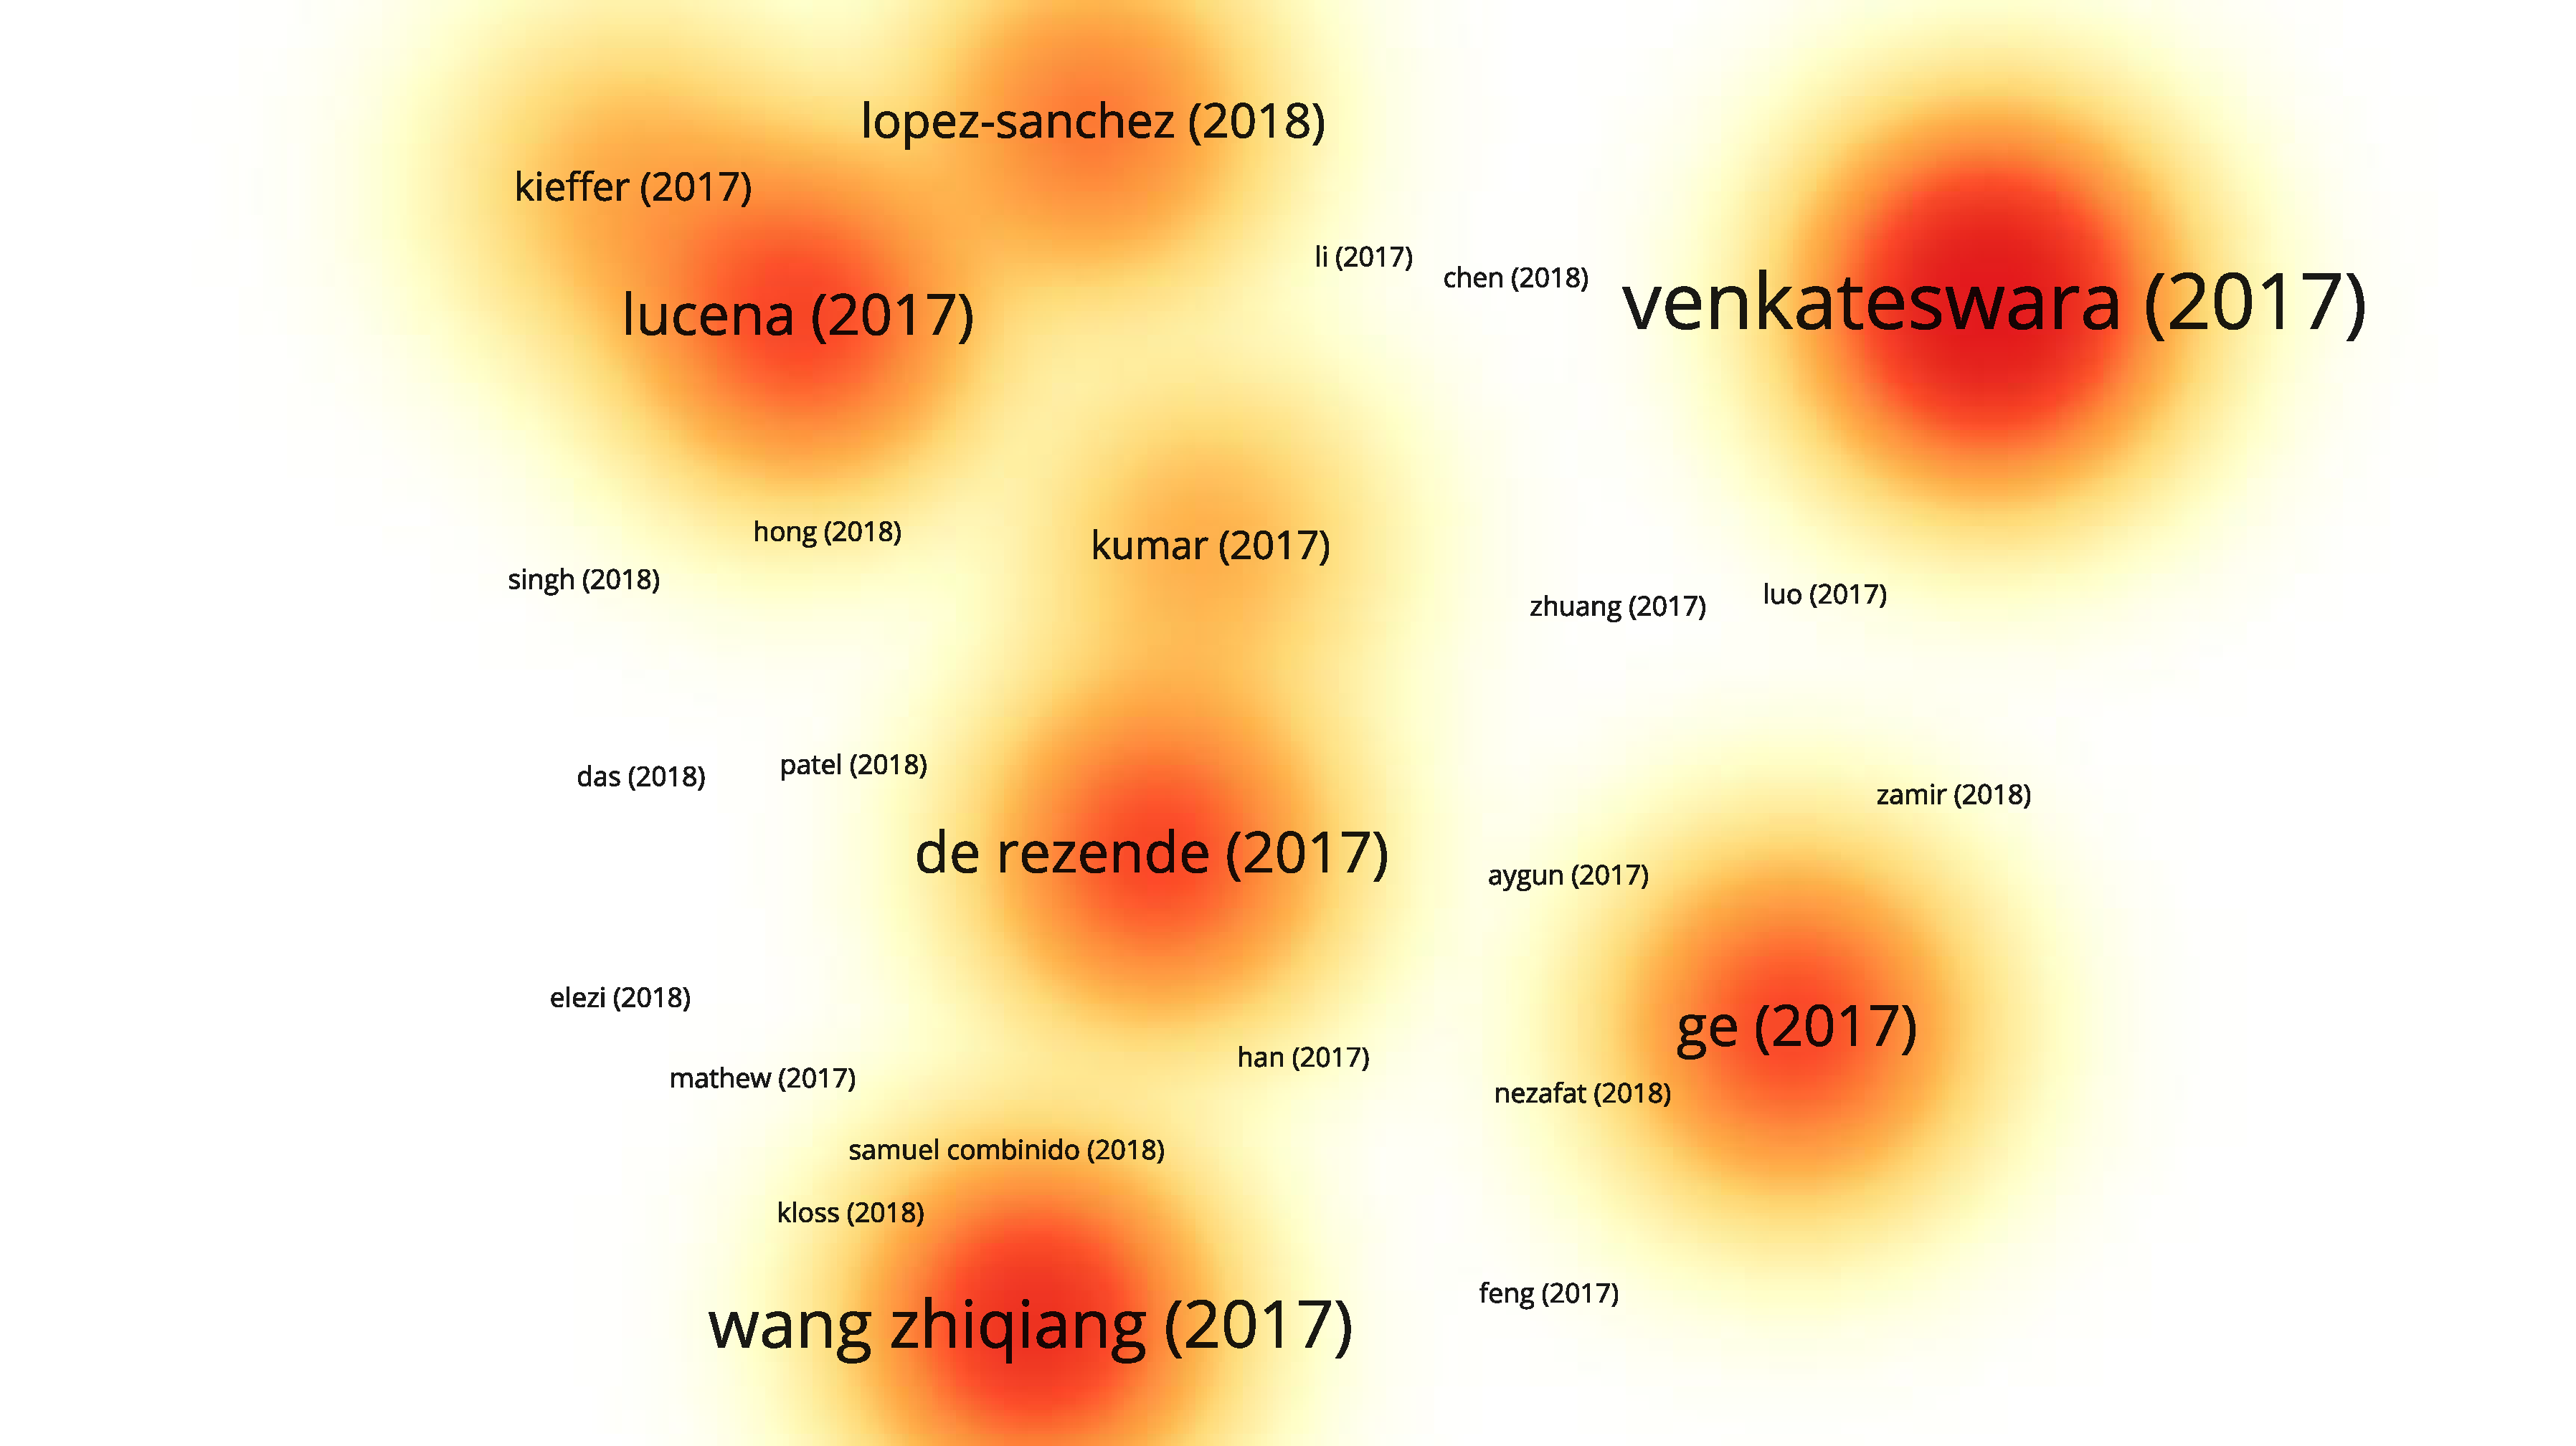
\includegraphics[width=\columnwidth]{frontier_heat}}
    \caption{} \label{fig:bicoupling}
  \end{figure}

\section{Problemas em Aberto}
\begin{enumerate}
  \item inexistência de métricas específicas para medir transferência.
  \item não há uma categorização que dê a devida importância a métodos mais novos (GANs, autoencoders)...???
  \item NLP
  \item Teoria
  \item categorização específica deep transfer learning
  \item 
\end{enumerate}
\lipsum[3]
\section{Conclusão}
\lipsum[3]
\bibliographystyle{ACM-Reference-Format}
\bibliography{references}
\end{document}
